\documentclass{beamer}
\usepackage[latin1]{inputenc}
%\usetheme{Montpellier}
\usetheme{Boadilla}
%\usecolortheme[RGB={204,51,255}]{structure}
%\usecolortheme[named=purple]{structure}
\usecolortheme[RGB={62,128,62}]{structure}
%\definecolor{dark}{rgb}{0.3,0.15,0.3}
%\definecolor{light}{rgb}{0.8,0.6,0.8}
%\definecolor{reddish}{rgb}{.5,0.15,0.15}
\definecolor{dark}{rgb}{0.4,0.2,0.4}
%\definecolor{light}{rgb}{0.8,0.6,0.8}
\definecolor{reddish}{rgb}{.7,0.25,0.25}
\usepackage{graphicx}
\usepackage{pstricks}

\usepackage{tikz}
\usetikzlibrary{arrows,decorations.markings,positioning}
\usepackage{epstopdf}

\title[Mutual information for functions.]{Mutual information for functions, maybe even ERPs.}
\author{Conor Houghton}
\institute{CS, U Bristol}
\date{Frankfurt, May 2018}

\begin{document}

\maketitle



\begin{frame}{Shannon's Entropy 1}
\color{dark}
$$
H(X)=-\sum_x p(x)\log_2{p(x)}
$$
\color{black}
\end{frame}



\begin{frame}{Shannon's Entropy 2}
\color{black}
\begin{center}
\begin{tabular}{cccccccc}
1/2&1/4&1/8&1/16&1/32&1/64&1/128&1/128\\
000&001&010&011&100&101&110&111\\
0&10&110&1110&11110&111110&1111110&1111111
\end{tabular}
\end{center}
\color{dark}
$$
\mbox{average code length}=\frac{1}{2}+\frac{1}{4}2+\frac{1}{8}3+\frac{1}{16}4+\ldots = H(X)\approx 1.98 < 3
$$
\color{black}
\end{frame}


\begin{frame}{Mutual Information 1}
\color{dark}
$$
I(X,Y)=H(X)-H(X|Y)=H(Y)-H(Y|X)
$$
\color{black}
\end{frame}


\begin{frame}{Mutual Information 1}
\color{dark}
$$
I(X,Y)=H(X)-H(X|Y)=H(Y)-H(Y|X)
$$
\color{black}
\begin{center}
info in $X$=(info remaining in X if you know Y)+(mutual info)
\end{center}
\end{frame}

\begin{frame}{Mutual Information 2}
\color{dark}
$$
I(X,Y)=\sum_{x,y} p_{X,Y}(x,y) \log_2{\frac{p_{X,Y}(x,y)}{p_X(x)p_Y(y)}}
$$
\color{black}
\end{frame}

\begin{frame}{Functions}
\color{reddish}
\begin{center}
% GNUPLOT: LaTeX picture with Postscript
\begingroup
  \makeatletter
  \providecommand\color[2][]{%
    \GenericError{(gnuplot) \space\space\space\@spaces}{%
      Package color not loaded in conjunction with
      terminal option `colourtext'%
    }{See the gnuplot documentation for explanation.%
    }{Either use 'blacktext' in gnuplot or load the package
      color.sty in LaTeX.}%
    \renewcommand\color[2][]{}%
  }%
  \providecommand\includegraphics[2][]{%
    \GenericError{(gnuplot) \space\space\space\@spaces}{%
      Package graphicx or graphics not loaded%
    }{See the gnuplot documentation for explanation.%
    }{The gnuplot epslatex terminal needs graphicx.sty or graphics.sty.}%
    \renewcommand\includegraphics[2][]{}%
  }%
  \providecommand\rotatebox[2]{#2}%
  \@ifundefined{ifGPcolor}{%
    \newif\ifGPcolor
    \GPcolorfalse
  }{}%
  \@ifundefined{ifGPblacktext}{%
    \newif\ifGPblacktext
    \GPblacktexttrue
  }{}%
  % define a \g@addto@macro without @ in the name:
  \let\gplgaddtomacro\g@addto@macro
  % define empty templates for all commands taking text:
  \gdef\gplbacktext{}%
  \gdef\gplfronttext{}%
  \makeatother
  \ifGPblacktext
    % no textcolor at all
    \def\colorrgb#1{}%
    \def\colorgray#1{}%
  \else
    % gray or color?
    \ifGPcolor
      \def\colorrgb#1{\color[rgb]{#1}}%
      \def\colorgray#1{\color[gray]{#1}}%
      \expandafter\def\csname LTw\endcsname{\color{white}}%
      \expandafter\def\csname LTb\endcsname{\color{black}}%
      \expandafter\def\csname LTa\endcsname{\color{black}}%
      \expandafter\def\csname LT0\endcsname{\color[rgb]{1,0,0}}%
      \expandafter\def\csname LT1\endcsname{\color[rgb]{0,1,0}}%
      \expandafter\def\csname LT2\endcsname{\color[rgb]{0,0,1}}%
      \expandafter\def\csname LT3\endcsname{\color[rgb]{1,0,1}}%
      \expandafter\def\csname LT4\endcsname{\color[rgb]{0,1,1}}%
      \expandafter\def\csname LT5\endcsname{\color[rgb]{1,1,0}}%
      \expandafter\def\csname LT6\endcsname{\color[rgb]{0,0,0}}%
      \expandafter\def\csname LT7\endcsname{\color[rgb]{1,0.3,0}}%
      \expandafter\def\csname LT8\endcsname{\color[rgb]{0.5,0.5,0.5}}%
    \else
      % gray
      \def\colorrgb#1{\color{black}}%
      \def\colorgray#1{\color[gray]{#1}}%
      \expandafter\def\csname LTw\endcsname{\color{white}}%
      \expandafter\def\csname LTb\endcsname{\color{black}}%
      \expandafter\def\csname LTa\endcsname{\color{black}}%
      \expandafter\def\csname LT0\endcsname{\color{black}}%
      \expandafter\def\csname LT1\endcsname{\color{black}}%
      \expandafter\def\csname LT2\endcsname{\color{black}}%
      \expandafter\def\csname LT3\endcsname{\color{black}}%
      \expandafter\def\csname LT4\endcsname{\color{black}}%
      \expandafter\def\csname LT5\endcsname{\color{black}}%
      \expandafter\def\csname LT6\endcsname{\color{black}}%
      \expandafter\def\csname LT7\endcsname{\color{black}}%
      \expandafter\def\csname LT8\endcsname{\color{black}}%
    \fi
  \fi
  \setlength{\unitlength}{0.0500bp}%
  \begin{picture}(3240.00,2268.00)%
    \gplgaddtomacro\gplbacktext{%
      \csname LTb\endcsname%
      \put(682,769){\makebox(0,0)[r]{\strut{}-6}}%
      \put(682,1029){\makebox(0,0)[r]{\strut{}-4}}%
      \put(682,1289){\makebox(0,0)[r]{\strut{}-2}}%
      \put(682,1549){\makebox(0,0)[r]{\strut{} 0}}%
      \put(682,1809){\makebox(0,0)[r]{\strut{} 2}}%
      \put(814,484){\makebox(0,0){\strut{} 0}}%
      \put(1219,484){\makebox(0,0){\strut{} 0.1}}%
      \put(1624,484){\makebox(0,0){\strut{} 0.2}}%
      \put(2029,484){\makebox(0,0){\strut{} 0.3}}%
      \put(2434,484){\makebox(0,0){\strut{} 0.4}}%
      \put(2839,484){\makebox(0,0){\strut{} 0.5}}%
      \put(176,1354){\rotatebox{-270}{\makebox(0,0){\strut{}field strength}}}%
      \put(1828,154){\makebox(0,0){\strut{}time (ms)}}%
    }%
    \gplgaddtomacro\gplfronttext{%
    }%
    \gplbacktext
    \put(0,0){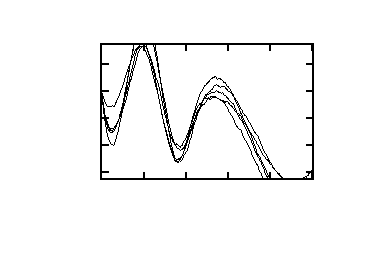
\includegraphics{example_erps_event_sigma2}}%
    \gplfronttext
  \end{picture}%
\endgroup

\end{center}
\end{frame}

\begin{frame}{A dart board 1}
\color{reddish}
\begin{center}
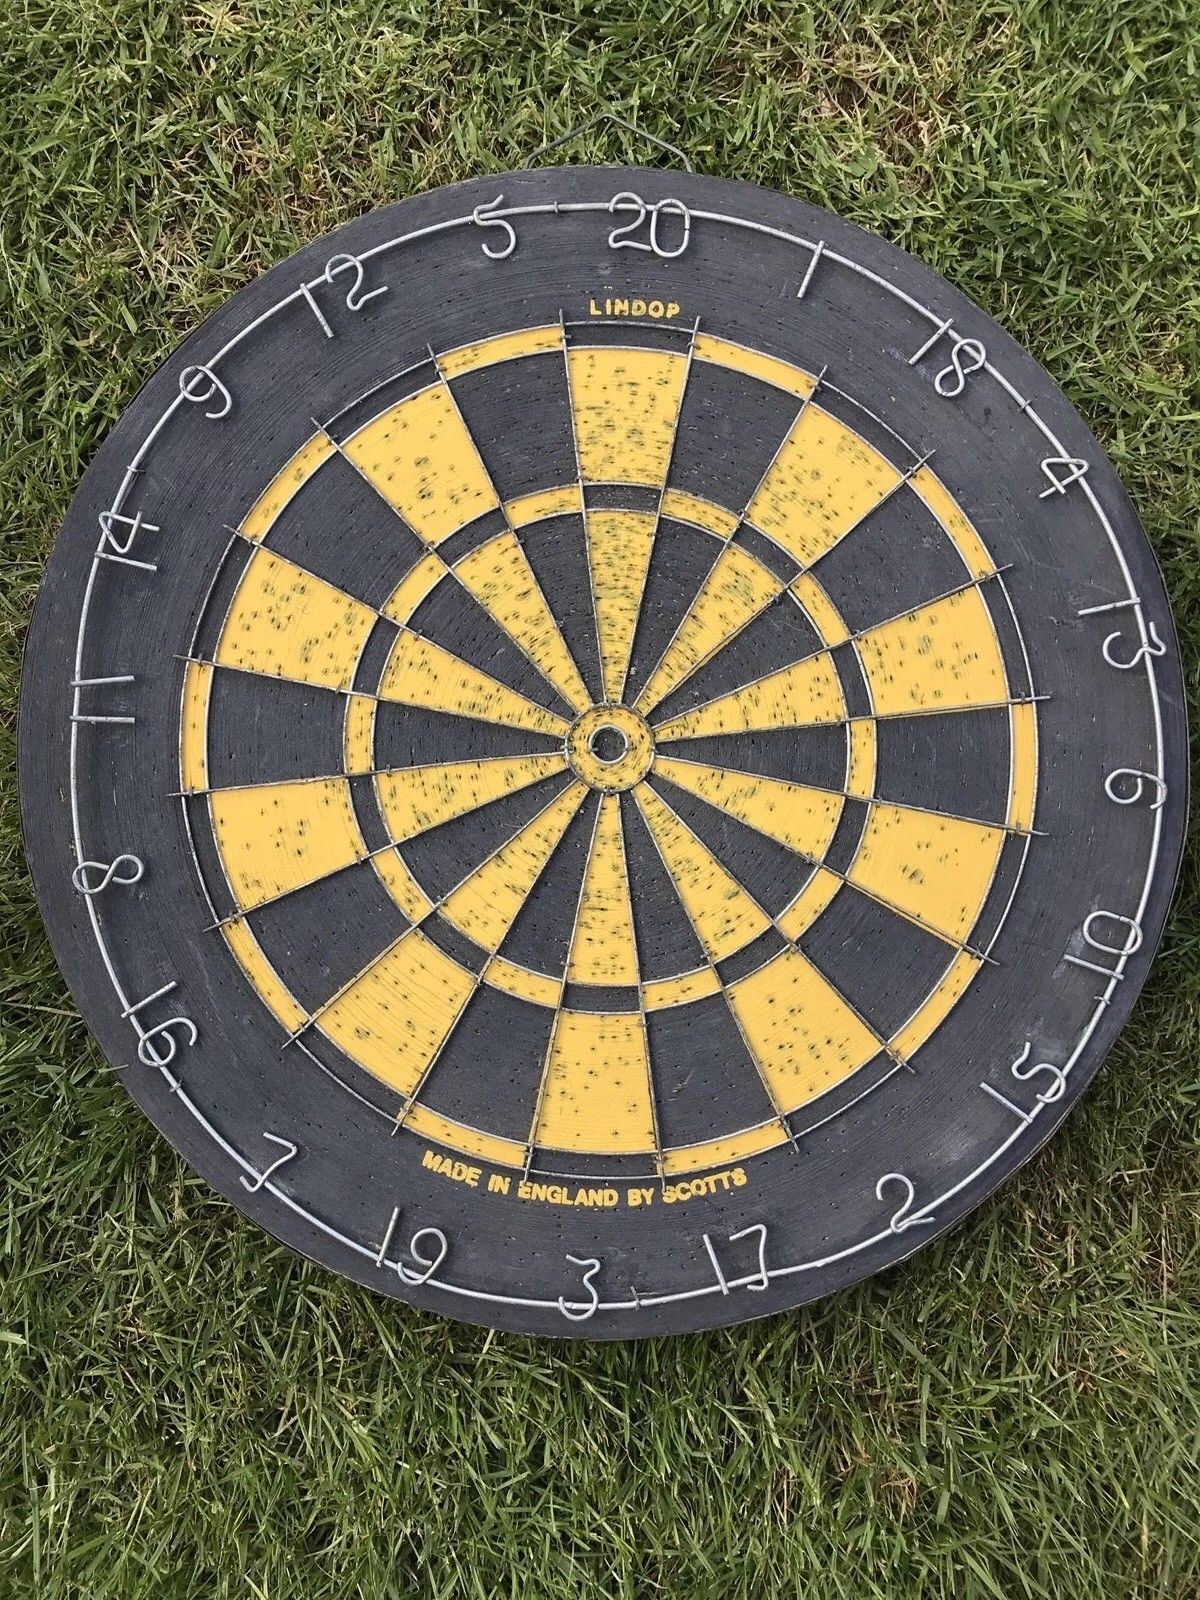
\includegraphics[width=4cm]{dart_board.jpg}
\end{center}
\color{black}
\vfill
\color{gray}
\flushright{\small{photo from ebay (\pounds 4.20 +p.p.)}}
\color{black}
\end{frame}

\begin{frame}{A dart board 2}
\color{reddish}
\begin{center}
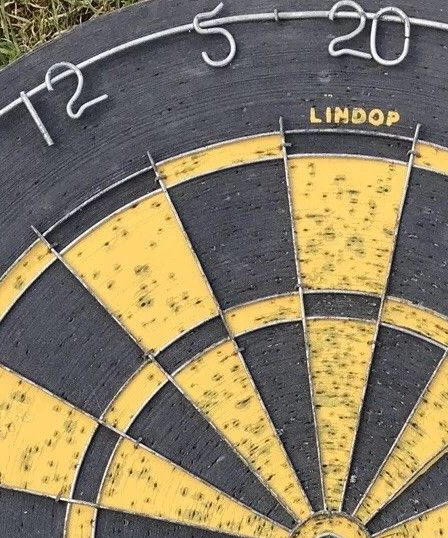
\includegraphics[width=4cm]{dart_board_zoom.png}
\end{center}
\color{black}
\end{frame}


\begin{frame}{Probability mass function}
\begin{center}
\includegraphics[width=4cm]{dart_board_region.png}
\end{center}
\color{dark}
$$\mbox{prob}(\mbox{dart lands in }B)=\int_B p(\mathbf{x})dV$$
\color{black}
\end{frame}


\begin{frame}{Estimating using the number of number of holes 1}
\color{reddish}
\begin{center}
\includegraphics[width=4cm]{dart_board_region.png}
\end{center}
\color{black}
$$\langle \mbox{number of holes in }B\rangle = \int_B p(\mathbf{x})dV \times (\mbox{total number of holes})$$
\end{frame}

\begin{frame}{Estimating using the number of number of holes 2}
\color{dark}
$$\mbox{vol}\,B\approx \frac{\mbox{number of holes in }B}{\mbox{total number of holes}}$$
\end{frame}

\begin{frame}{Estimating the probability mass function}
\color{black}
If the mass function varies slowly:
\color{dark}
$$\int_B p(\mathbf{x})dV\approx p(\mathbf{x}_0) \times \mbox{vol}\,B$$
\color{black}
so
\color{dark}
$$\mbox{number of holes in }B \approx p(\mathbf{x}_0) \times \mbox{vol}\,B \times (\mbox{total number of holes})$$
\color{black}
Using this to find the mutual information gives a \textsl{Kozachenko-Leonenko} estimator.
\end{frame}


\begin{frame}{Estimating using the number of number of holes 3}
\color{dark}
$$p(x_0)\approx%\frac{\#B}{n\times \mbox{vol}\,B}
$$
\color{black}
where $n$ is the total number of points and $\#B$ is the number of points in $B$.
\color{reddish}
\begin{center}
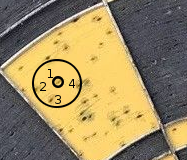
\includegraphics[width=4cm]{dart_board_zoom_ball.png}
\end{center}
\color{black}
so 
$$p(\circ)=\frac{4}{b\mbox{vol}\,B}$$
\end{frame}



\begin{frame}{Kozachenko-Leonenko estimators are very good}
\color{reddish}
\begin{center}
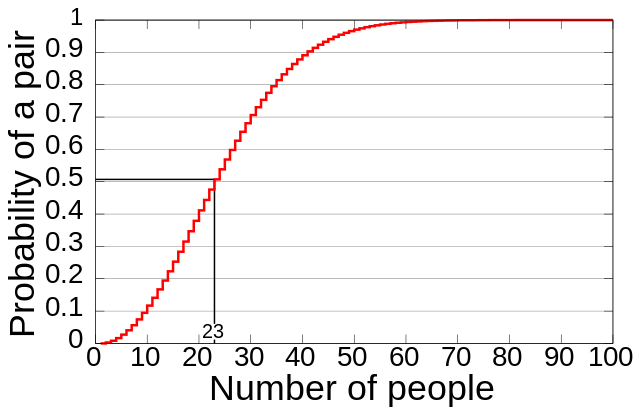
\includegraphics[width=6cm]{Birthday_Paradox.png}
\end{center}
\color{black}
\vfill
\color{gray}
\flushright{\small{graph from wikipedia article on the birthday paradox}}
\color{black}
\end{frame}



\begin{frame}{Problem}
\color{black}
How do we work out the volume in the space of functions? We have no coordinates $xyz$ to do
\color{dark}
$$\mbox{vol}\,B=\int_B dxdydz$$
\end{frame}

\begin{frame}{Use the mass function as a measure!}
\color{reddish}
\begin{center}
\includegraphics[width=4cm]{dart_board_big_20.png}
\end{center}
\color{dark}
$$\mbox{vol}\,B=\int_B p(\mathbf{x}) dV$$
\color{black}
\end{frame}


\begin{frame}{Volume by counting holes 1}
\color{dark}
$$\mbox{vol}\,B\approx \frac{\mbox{number of holes in }B}{\mbox{total number of holes}}$$
\end{frame}

\begin{frame}{Volume by counting holes 2}
\color{reddish}
\begin{center}
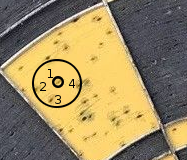
\includegraphics[width=4cm]{dart_board_zoom_ball.png}
\end{center}
\color{black}
A ball with volume $h/n$ around the circled point, where $n$ is the total number of holes and $h=4$.
\end{frame}


\begin{frame}{Metric}
To make a ball you need a metric; not to measure the radius since the
size is being defined by the volume, but to define \lq{}the nearest
$h$ points\rq{}.
\color{reddish}
\begin{center}
\color{reddish}
% GNUPLOT: LaTeX picture with Postscript
\begingroup
  \makeatletter
  \providecommand\color[2][]{%
    \GenericError{(gnuplot) \space\space\space\@spaces}{%
      Package color not loaded in conjunction with
      terminal option `colourtext'%
    }{See the gnuplot documentation for explanation.%
    }{Either use 'blacktext' in gnuplot or load the package
      color.sty in LaTeX.}%
    \renewcommand\color[2][]{}%
  }%
  \providecommand\includegraphics[2][]{%
    \GenericError{(gnuplot) \space\space\space\@spaces}{%
      Package graphicx or graphics not loaded%
    }{See the gnuplot documentation for explanation.%
    }{The gnuplot epslatex terminal needs graphicx.sty or graphics.sty.}%
    \renewcommand\includegraphics[2][]{}%
  }%
  \providecommand\rotatebox[2]{#2}%
  \@ifundefined{ifGPcolor}{%
    \newif\ifGPcolor
    \GPcolorfalse
  }{}%
  \@ifundefined{ifGPblacktext}{%
    \newif\ifGPblacktext
    \GPblacktexttrue
  }{}%
  % define a \g@addto@macro without @ in the name:
  \let\gplgaddtomacro\g@addto@macro
  % define empty templates for all commands taking text:
  \gdef\gplbacktext{}%
  \gdef\gplfronttext{}%
  \makeatother
  \ifGPblacktext
    % no textcolor at all
    \def\colorrgb#1{}%
    \def\colorgray#1{}%
  \else
    % gray or color?
    \ifGPcolor
      \def\colorrgb#1{\color[rgb]{#1}}%
      \def\colorgray#1{\color[gray]{#1}}%
      \expandafter\def\csname LTw\endcsname{\color{white}}%
      \expandafter\def\csname LTb\endcsname{\color{black}}%
      \expandafter\def\csname LTa\endcsname{\color{black}}%
      \expandafter\def\csname LT0\endcsname{\color[rgb]{1,0,0}}%
      \expandafter\def\csname LT1\endcsname{\color[rgb]{0,1,0}}%
      \expandafter\def\csname LT2\endcsname{\color[rgb]{0,0,1}}%
      \expandafter\def\csname LT3\endcsname{\color[rgb]{1,0,1}}%
      \expandafter\def\csname LT4\endcsname{\color[rgb]{0,1,1}}%
      \expandafter\def\csname LT5\endcsname{\color[rgb]{1,1,0}}%
      \expandafter\def\csname LT6\endcsname{\color[rgb]{0,0,0}}%
      \expandafter\def\csname LT7\endcsname{\color[rgb]{1,0.3,0}}%
      \expandafter\def\csname LT8\endcsname{\color[rgb]{0.5,0.5,0.5}}%
    \else
      % gray
      \def\colorrgb#1{\color{black}}%
      \def\colorgray#1{\color[gray]{#1}}%
      \expandafter\def\csname LTw\endcsname{\color{white}}%
      \expandafter\def\csname LTb\endcsname{\color{black}}%
      \expandafter\def\csname LTa\endcsname{\color{black}}%
      \expandafter\def\csname LT0\endcsname{\color{black}}%
      \expandafter\def\csname LT1\endcsname{\color{black}}%
      \expandafter\def\csname LT2\endcsname{\color{black}}%
      \expandafter\def\csname LT3\endcsname{\color{black}}%
      \expandafter\def\csname LT4\endcsname{\color{black}}%
      \expandafter\def\csname LT5\endcsname{\color{black}}%
      \expandafter\def\csname LT6\endcsname{\color{black}}%
      \expandafter\def\csname LT7\endcsname{\color{black}}%
      \expandafter\def\csname LT8\endcsname{\color{black}}%
    \fi
  \fi
  \setlength{\unitlength}{0.0500bp}%
  \begin{picture}(4320.00,3024.00)%
    \gplgaddtomacro\gplbacktext{%
      \csname LTb\endcsname%
      \put(682,790){\makebox(0,0)[r]{\strut{}-8}}%
      \put(682,1132){\makebox(0,0)[r]{\strut{}-6}}%
      \put(682,1475){\makebox(0,0)[r]{\strut{}-4}}%
      \put(682,1817){\makebox(0,0)[r]{\strut{}-2}}%
      \put(682,2160){\makebox(0,0)[r]{\strut{} 0}}%
      \put(682,2502){\makebox(0,0)[r]{\strut{} 2}}%
      \put(820,484){\makebox(0,0){\strut{} 0}}%
      \put(1440,484){\makebox(0,0){\strut{} 0.1}}%
      \put(2059,484){\makebox(0,0){\strut{} 0.2}}%
      \put(2678,484){\makebox(0,0){\strut{} 0.3}}%
      \put(3297,484){\makebox(0,0){\strut{} 0.4}}%
      \put(3917,484){\makebox(0,0){\strut{} 0.5}}%
      \put(176,1731){\rotatebox{-270}{\makebox(0,0){\strut{}field strength}}}%
      \put(2368,154){\makebox(0,0){\strut{}time (ms)}}%
    }%
    \gplgaddtomacro\gplfronttext{%
    }%
    \gplbacktext
    \put(0,0){\includegraphics{two_erps}}%
    \gplfronttext
  \end{picture}%
\endgroup

\end{center}
\end{frame}


\begin{frame}{Oh no}
$$p(\mathbf{x}_0)\approx\frac{\#B}{n\times \mbox{vol}\,B}=\frac{h}{nh/n}=1$$
and using this meaure gives $H(X)=0$; in fact the
  differential entropy is not well-defined. However the
  mutual information is!
\end{frame}


\begin{frame}{Mutual infomation}
$$I(X,Y)=H(Y)-H(Y|X)$$ has two probability distributions: $p_Y(y)$ and
  $p_{Y|X}(y|x)$! IDEA: use one to estimate volume, the other can then
  be estimated by counting!
\end{frame}

\begin{frame}{Formula}
This is for the case where $X$ is a discrete random variable and
everything exciting is happening in $Y$ space.
$$I(X,Y)=\frac{1}{n}\sum_{y_i}\log_2{\frac{n\#_{y_i}B}{h}}$$
where $\#_{x}B$ are the number of points in $B$ that correspond to the $X$ value.
\end{frame}


\begin{frame}{h}

There are two approximations:
$$\int_B p(x)dV = \# B\times \mbox{vol}\,B$$
and
$$\int_B p(x)dV = \mbox{V}\times p(x_0)$$ 

The first approximation gets better if the volume is bigger, the
second gets worse; the correct choice of $h$ is a compromize between
these two. There is actually a clever approach to picking $h$ that
seems to work, based on the bias.
\end{frame}


\begin{frame}{Pretend ERPs 1}
\color{reddish}
\begin{center}
% GNUPLOT: LaTeX picture with Postscript
\begingroup
  \makeatletter
  \providecommand\color[2][]{%
    \GenericError{(gnuplot) \space\space\space\@spaces}{%
      Package color not loaded in conjunction with
      terminal option `colourtext'%
    }{See the gnuplot documentation for explanation.%
    }{Either use 'blacktext' in gnuplot or load the package
      color.sty in LaTeX.}%
    \renewcommand\color[2][]{}%
  }%
  \providecommand\includegraphics[2][]{%
    \GenericError{(gnuplot) \space\space\space\@spaces}{%
      Package graphicx or graphics not loaded%
    }{See the gnuplot documentation for explanation.%
    }{The gnuplot epslatex terminal needs graphicx.sty or graphics.sty.}%
    \renewcommand\includegraphics[2][]{}%
  }%
  \providecommand\rotatebox[2]{#2}%
  \@ifundefined{ifGPcolor}{%
    \newif\ifGPcolor
    \GPcolorfalse
  }{}%
  \@ifundefined{ifGPblacktext}{%
    \newif\ifGPblacktext
    \GPblacktexttrue
  }{}%
  % define a \g@addto@macro without @ in the name:
  \let\gplgaddtomacro\g@addto@macro
  % define empty templates for all commands taking text:
  \gdef\gplbacktext{}%
  \gdef\gplfronttext{}%
  \makeatother
  \ifGPblacktext
    % no textcolor at all
    \def\colorrgb#1{}%
    \def\colorgray#1{}%
  \else
    % gray or color?
    \ifGPcolor
      \def\colorrgb#1{\color[rgb]{#1}}%
      \def\colorgray#1{\color[gray]{#1}}%
      \expandafter\def\csname LTw\endcsname{\color{white}}%
      \expandafter\def\csname LTb\endcsname{\color{black}}%
      \expandafter\def\csname LTa\endcsname{\color{black}}%
      \expandafter\def\csname LT0\endcsname{\color[rgb]{1,0,0}}%
      \expandafter\def\csname LT1\endcsname{\color[rgb]{0,1,0}}%
      \expandafter\def\csname LT2\endcsname{\color[rgb]{0,0,1}}%
      \expandafter\def\csname LT3\endcsname{\color[rgb]{1,0,1}}%
      \expandafter\def\csname LT4\endcsname{\color[rgb]{0,1,1}}%
      \expandafter\def\csname LT5\endcsname{\color[rgb]{1,1,0}}%
      \expandafter\def\csname LT6\endcsname{\color[rgb]{0,0,0}}%
      \expandafter\def\csname LT7\endcsname{\color[rgb]{1,0.3,0}}%
      \expandafter\def\csname LT8\endcsname{\color[rgb]{0.5,0.5,0.5}}%
    \else
      % gray
      \def\colorrgb#1{\color{black}}%
      \def\colorgray#1{\color[gray]{#1}}%
      \expandafter\def\csname LTw\endcsname{\color{white}}%
      \expandafter\def\csname LTb\endcsname{\color{black}}%
      \expandafter\def\csname LTa\endcsname{\color{black}}%
      \expandafter\def\csname LT0\endcsname{\color{black}}%
      \expandafter\def\csname LT1\endcsname{\color{black}}%
      \expandafter\def\csname LT2\endcsname{\color{black}}%
      \expandafter\def\csname LT3\endcsname{\color{black}}%
      \expandafter\def\csname LT4\endcsname{\color{black}}%
      \expandafter\def\csname LT5\endcsname{\color{black}}%
      \expandafter\def\csname LT6\endcsname{\color{black}}%
      \expandafter\def\csname LT7\endcsname{\color{black}}%
      \expandafter\def\csname LT8\endcsname{\color{black}}%
    \fi
  \fi
  \setlength{\unitlength}{0.0500bp}%
  \begin{picture}(6240.00,2268.00)%
    \gplgaddtomacro\gplbacktext{%
      \csname LTb\endcsname%
      \put(682,769){\makebox(0,0)[r]{\strut{}-6}}%
      \put(682,1029){\makebox(0,0)[r]{\strut{}-4}}%
      \put(682,1289){\makebox(0,0)[r]{\strut{}-2}}%
      \put(682,1549){\makebox(0,0)[r]{\strut{} 0}}%
      \put(682,1809){\makebox(0,0)[r]{\strut{} 2}}%
      \put(818,484){\makebox(0,0){\strut{} 0}}%
      \put(1222,484){\makebox(0,0){\strut{} 0.1}}%
      \put(1626,484){\makebox(0,0){\strut{} 0.2}}%
      \put(2031,484){\makebox(0,0){\strut{} 0.3}}%
      \put(2435,484){\makebox(0,0){\strut{} 0.4}}%
      \put(2839,484){\makebox(0,0){\strut{} 0.5}}%
      \put(176,1354){\rotatebox{-270}{\makebox(0,0){\strut{}field strength}}}%
      \put(1828,154){\makebox(0,0){\strut{}time (ms)}}%
      \put(3682,769){\makebox(0,0)[r]{\strut{}-6}}%
      \put(3682,1029){\makebox(0,0)[r]{\strut{}-4}}%
      \put(3682,1289){\makebox(0,0)[r]{\strut{}-2}}%
      \put(3682,1549){\makebox(0,0)[r]{\strut{} 0}}%
      \put(3682,1809){\makebox(0,0)[r]{\strut{} 2}}%
      \put(3818,484){\makebox(0,0){\strut{} 0}}%
      \put(4222,484){\makebox(0,0){\strut{} 0.1}}%
      \put(4626,484){\makebox(0,0){\strut{} 0.2}}%
      \put(5031,484){\makebox(0,0){\strut{} 0.3}}%
      \put(5435,484){\makebox(0,0){\strut{} 0.4}}%
      \put(5839,484){\makebox(0,0){\strut{} 0.5}}%
      \put(4828,154){\makebox(0,0){\strut{}time (ms)}}%
    }%
    \gplgaddtomacro\gplfronttext{%
    }%
    \gplbacktext
    \put(0,2300){\makebox(0,0){\strut{}\textbf{A}}}%
    \put(3200,2300){\makebox(0,0){\strut{}\textbf{B}}}%
    \put(3000,0){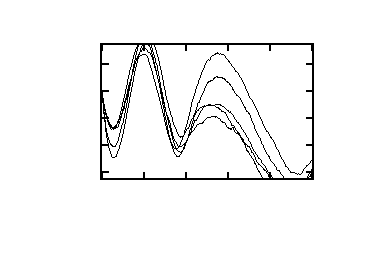
\includegraphics{example_erp_events}}%
    \put(0,0){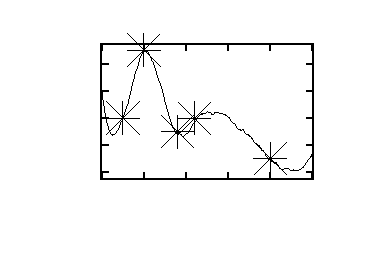
\includegraphics{example_erp}}%
    \gplfronttext
  \end{picture}%
\endgroup

\end{center}
\color{black} \textbf{Fictive event related potentials.} The
\lq{}stimuli\rq{} are random 5-vectors of landmarks; an ERP is
produces by perturbing the landmarks, interpolating with splines and
adding noise. \textbf{B} shows responses to different stimuli.
\color{black}
\end{frame}


\begin{frame}{Pretend ERPs 2}
\color{reddish}
\begin{center}
% GNUPLOT: LaTeX picture with Postscript
\begingroup
  \makeatletter
  \providecommand\color[2][]{%
    \GenericError{(gnuplot) \space\space\space\@spaces}{%
      Package color not loaded in conjunction with
      terminal option `colourtext'%
    }{See the gnuplot documentation for explanation.%
    }{Either use 'blacktext' in gnuplot or load the package
      color.sty in LaTeX.}%
    \renewcommand\color[2][]{}%
  }%
  \providecommand\includegraphics[2][]{%
    \GenericError{(gnuplot) \space\space\space\@spaces}{%
      Package graphicx or graphics not loaded%
    }{See the gnuplot documentation for explanation.%
    }{The gnuplot epslatex terminal needs graphicx.sty or graphics.sty.}%
    \renewcommand\includegraphics[2][]{}%
  }%
  \providecommand\rotatebox[2]{#2}%
  \@ifundefined{ifGPcolor}{%
    \newif\ifGPcolor
    \GPcolorfalse
  }{}%
  \@ifundefined{ifGPblacktext}{%
    \newif\ifGPblacktext
    \GPblacktexttrue
  }{}%
  % define a \g@addto@macro without @ in the name:
  \let\gplgaddtomacro\g@addto@macro
  % define empty templates for all commands taking text:
  \gdef\gplbacktext{}%
  \gdef\gplfronttext{}%
  \makeatother
  \ifGPblacktext
    % no textcolor at all
    \def\colorrgb#1{}%
    \def\colorgray#1{}%
  \else
    % gray or color?
    \ifGPcolor
      \def\colorrgb#1{\color[rgb]{#1}}%
      \def\colorgray#1{\color[gray]{#1}}%
      \expandafter\def\csname LTw\endcsname{\color{white}}%
      \expandafter\def\csname LTb\endcsname{\color{black}}%
      \expandafter\def\csname LTa\endcsname{\color{black}}%
      \expandafter\def\csname LT0\endcsname{\color[rgb]{1,0,0}}%
      \expandafter\def\csname LT1\endcsname{\color[rgb]{0,1,0}}%
      \expandafter\def\csname LT2\endcsname{\color[rgb]{0,0,1}}%
      \expandafter\def\csname LT3\endcsname{\color[rgb]{1,0,1}}%
      \expandafter\def\csname LT4\endcsname{\color[rgb]{0,1,1}}%
      \expandafter\def\csname LT5\endcsname{\color[rgb]{1,1,0}}%
      \expandafter\def\csname LT6\endcsname{\color[rgb]{0,0,0}}%
      \expandafter\def\csname LT7\endcsname{\color[rgb]{1,0.3,0}}%
      \expandafter\def\csname LT8\endcsname{\color[rgb]{0.5,0.5,0.5}}%
    \else
      % gray
      \def\colorrgb#1{\color{black}}%
      \def\colorgray#1{\color[gray]{#1}}%
      \expandafter\def\csname LTw\endcsname{\color{white}}%
      \expandafter\def\csname LTb\endcsname{\color{black}}%
      \expandafter\def\csname LTa\endcsname{\color{black}}%
      \expandafter\def\csname LT0\endcsname{\color{black}}%
      \expandafter\def\csname LT1\endcsname{\color{black}}%
      \expandafter\def\csname LT2\endcsname{\color{black}}%
      \expandafter\def\csname LT3\endcsname{\color{black}}%
      \expandafter\def\csname LT4\endcsname{\color{black}}%
      \expandafter\def\csname LT5\endcsname{\color{black}}%
      \expandafter\def\csname LT6\endcsname{\color{black}}%
      \expandafter\def\csname LT7\endcsname{\color{black}}%
      \expandafter\def\csname LT8\endcsname{\color{black}}%
    \fi
  \fi
  \setlength{\unitlength}{0.0500bp}%
  \begin{picture}(6240.00,2268.00)%
    \gplgaddtomacro\gplbacktext{%
      \csname LTb\endcsname%
      \put(682,769){\makebox(0,0)[r]{\strut{}-6}}%
      \put(682,1029){\makebox(0,0)[r]{\strut{}-4}}%
      \put(682,1289){\makebox(0,0)[r]{\strut{}-2}}%
      \put(682,1549){\makebox(0,0)[r]{\strut{} 0}}%
      \put(682,1809){\makebox(0,0)[r]{\strut{} 2}}%
      \put(814,484){\makebox(0,0){\strut{} 0}}%
      \put(1219,484){\makebox(0,0){\strut{} 0.1}}%
      \put(1624,484){\makebox(0,0){\strut{} 0.2}}%
      \put(2029,484){\makebox(0,0){\strut{} 0.3}}%
      \put(2434,484){\makebox(0,0){\strut{} 0.4}}%
      \put(2839,484){\makebox(0,0){\strut{} 0.5}}%
      \put(176,1354){\rotatebox{-270}{\makebox(0,0){\strut{}field strength}}}%
      \put(1828,154){\makebox(0,0){\strut{}time (ms)}}%
      \put(3682,769){\makebox(0,0)[r]{\strut{}-6}}%
      \put(3682,1029){\makebox(0,0)[r]{\strut{}-4}}%
      \put(3682,1289){\makebox(0,0)[r]{\strut{}-2}}%
      \put(3682,1549){\makebox(0,0)[r]{\strut{} 0}}%
      \put(3682,1809){\makebox(0,0)[r]{\strut{} 2}}%
      \put(3814,484){\makebox(0,0){\strut{} 0}}%
      \put(4219,484){\makebox(0,0){\strut{} 0.1}}%
      \put(4624,484){\makebox(0,0){\strut{} 0.2}}%
      \put(5029,484){\makebox(0,0){\strut{} 0.3}}%
      \put(5434,484){\makebox(0,0){\strut{} 0.4}}%
      \put(5839,484){\makebox(0,0){\strut{} 0.5}}%
      \put(4828,154){\makebox(0,0){\strut{}time (ms)}}%
    }%
    \gplgaddtomacro\gplfronttext{%
    }%
    \gplbacktext
    \put(0,2300){\makebox(0,0){\strut{}\textbf{A}}}%
    \put(3200,2300){\makebox(0,0){\strut{}\textbf{B}}}%
    \put(0,0){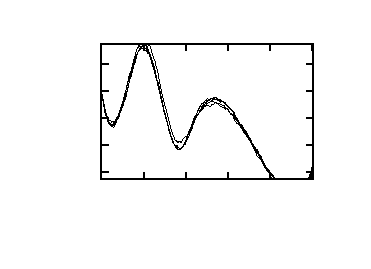
\includegraphics{example_erps_event_sigma0}}%
    \put(3000,0){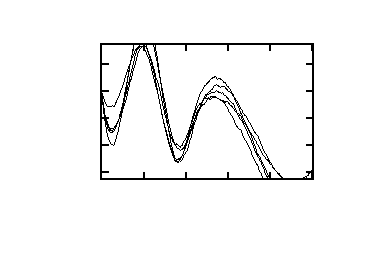
\includegraphics{example_erps_event_sigma2}}%
    \gplfronttext
  \end{picture}%
\endgroup

\end{center}
\color{black} \textbf{Multiple trials to the same stimulus.} The
amount the landmark points are moved is determined by $\sigma$; for
\textbf{A} $\sigma=0.0$, for \textbf{B} $\sigma=2$.  \color{black}
\end{frame}



\begin{frame}{Results 1}
\color{reddish}
\begin{center}
% GNUPLOT: LaTeX picture with Postscript
\begingroup
  \makeatletter
  \providecommand\color[2][]{%
    \GenericError{(gnuplot) \space\space\space\@spaces}{%
      Package color not loaded in conjunction with
      terminal option `colourtext'%
    }{See the gnuplot documentation for explanation.%
    }{Either use 'blacktext' in gnuplot or load the package
      color.sty in LaTeX.}%
    \renewcommand\color[2][]{}%
  }%
  \providecommand\includegraphics[2][]{%
    \GenericError{(gnuplot) \space\space\space\@spaces}{%
      Package graphicx or graphics not loaded%
    }{See the gnuplot documentation for explanation.%
    }{The gnuplot epslatex terminal needs graphicx.sty or graphics.sty.}%
    \renewcommand\includegraphics[2][]{}%
  }%
  \providecommand\rotatebox[2]{#2}%
  \@ifundefined{ifGPcolor}{%
    \newif\ifGPcolor
    \GPcolorfalse
  }{}%
  \@ifundefined{ifGPblacktext}{%
    \newif\ifGPblacktext
    \GPblacktexttrue
  }{}%
  % define a \g@addto@macro without @ in the name:
  \let\gplgaddtomacro\g@addto@macro
  % define empty templates for all commands taking text:
  \gdef\gplbacktext{}%
  \gdef\gplfronttext{}%
  \makeatother
  \ifGPblacktext
    % no textcolor at all
    \def\colorrgb#1{}%
    \def\colorgray#1{}%
  \else
    % gray or color?
    \ifGPcolor
      \def\colorrgb#1{\color[rgb]{#1}}%
      \def\colorgray#1{\color[gray]{#1}}%
      \expandafter\def\csname LTw\endcsname{\color{white}}%
      \expandafter\def\csname LTb\endcsname{\color{black}}%
      \expandafter\def\csname LTa\endcsname{\color{black}}%
      \expandafter\def\csname LT0\endcsname{\color[rgb]{1,0,0}}%
      \expandafter\def\csname LT1\endcsname{\color[rgb]{0,1,0}}%
      \expandafter\def\csname LT2\endcsname{\color[rgb]{0,0,1}}%
      \expandafter\def\csname LT3\endcsname{\color[rgb]{1,0,1}}%
      \expandafter\def\csname LT4\endcsname{\color[rgb]{0,1,1}}%
      \expandafter\def\csname LT5\endcsname{\color[rgb]{1,1,0}}%
      \expandafter\def\csname LT6\endcsname{\color[rgb]{0,0,0}}%
      \expandafter\def\csname LT7\endcsname{\color[rgb]{1,0.3,0}}%
      \expandafter\def\csname LT8\endcsname{\color[rgb]{0.5,0.5,0.5}}%
    \else
      % gray
      \def\colorrgb#1{\color{black}}%
      \def\colorgray#1{\color[gray]{#1}}%
      \expandafter\def\csname LTw\endcsname{\color{white}}%
      \expandafter\def\csname LTb\endcsname{\color{black}}%
      \expandafter\def\csname LTa\endcsname{\color{black}}%
      \expandafter\def\csname LT0\endcsname{\color{black}}%
      \expandafter\def\csname LT1\endcsname{\color{black}}%
      \expandafter\def\csname LT2\endcsname{\color{black}}%
      \expandafter\def\csname LT3\endcsname{\color{black}}%
      \expandafter\def\csname LT4\endcsname{\color{black}}%
      \expandafter\def\csname LT5\endcsname{\color{black}}%
      \expandafter\def\csname LT6\endcsname{\color{black}}%
      \expandafter\def\csname LT7\endcsname{\color{black}}%
      \expandafter\def\csname LT8\endcsname{\color{black}}%
    \fi
  \fi
  \setlength{\unitlength}{0.0500bp}%
  \begin{picture}(4320.00,3024.00)%
    \gplgaddtomacro\gplbacktext{%
      \csname LTb\endcsname%
      \put(946,704){\makebox(0,0)[r]{\strut{} 0}}%
      \put(946,998){\makebox(0,0)[r]{\strut{} 0.5}}%
      \put(946,1291){\makebox(0,0)[r]{\strut{} 1}}%
      \put(946,1585){\makebox(0,0)[r]{\strut{} 1.5}}%
      \put(946,1878){\makebox(0,0)[r]{\strut{} 2}}%
      \put(946,2172){\makebox(0,0)[r]{\strut{} 2.5}}%
      \put(946,2465){\makebox(0,0)[r]{\strut{} 3}}%
      \put(946,2759){\makebox(0,0)[r]{\strut{} 3.5}}%
      \put(1078,484){\makebox(0,0){\strut{} 0}}%
      \put(1647,484){\makebox(0,0){\strut{} 1}}%
      \put(2216,484){\makebox(0,0){\strut{} 2}}%
      \put(2785,484){\makebox(0,0){\strut{} 3}}%
      \put(3354,484){\makebox(0,0){\strut{} 4}}%
      \put(3923,484){\makebox(0,0){\strut{} 5}}%
      \put(176,1731){\rotatebox{-270}{\makebox(0,0){\strut{}mutual information (bits)}}}%
      \put(2500,154){\makebox(0,0){\strut{}$\sigma$}}%
    }%
    \gplgaddtomacro\gplfronttext{%
      \csname LTb\endcsname%
      \put(2936,2586){\makebox(0,0)[r]{\strut{}200 trials}}%
      \csname LTb\endcsname%
      \put(2936,2366){\makebox(0,0)[r]{\strut{}20 trials}}%
    }%
    \gplbacktext
    \put(0,0){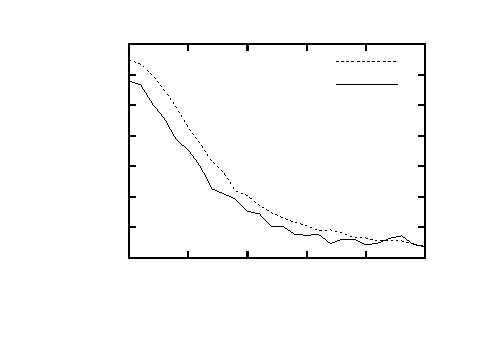
\includegraphics{info_v_event_sigma_plot}}%
    \gplfronttext
  \end{picture}%
\endgroup

\color{black} \textbf{Estimated mutual information.} \color{black}
\end{center}
\end{frame}


\begin{frame}{Results 2}
\color{reddish}
\begin{center}
  % GNUPLOT: LaTeX picture with Postscript
\begingroup
  \makeatletter
  \providecommand\color[2][]{%
    \GenericError{(gnuplot) \space\space\space\@spaces}{%
      Package color not loaded in conjunction with
      terminal option `colourtext'%
    }{See the gnuplot documentation for explanation.%
    }{Either use 'blacktext' in gnuplot or load the package
      color.sty in LaTeX.}%
    \renewcommand\color[2][]{}%
  }%
  \providecommand\includegraphics[2][]{%
    \GenericError{(gnuplot) \space\space\space\@spaces}{%
      Package graphicx or graphics not loaded%
    }{See the gnuplot documentation for explanation.%
    }{The gnuplot epslatex terminal needs graphicx.sty or graphics.sty.}%
    \renewcommand\includegraphics[2][]{}%
  }%
  \providecommand\rotatebox[2]{#2}%
  \@ifundefined{ifGPcolor}{%
    \newif\ifGPcolor
    \GPcolorfalse
  }{}%
  \@ifundefined{ifGPblacktext}{%
    \newif\ifGPblacktext
    \GPblacktexttrue
  }{}%
  % define a \g@addto@macro without @ in the name:
  \let\gplgaddtomacro\g@addto@macro
  % define empty templates for all commands taking text:
  \gdef\gplbacktext{}%
  \gdef\gplfronttext{}%
  \makeatother
  \ifGPblacktext
    % no textcolor at all
    \def\colorrgb#1{}%
    \def\colorgray#1{}%
  \else
    % gray or color?
    \ifGPcolor
      \def\colorrgb#1{\color[rgb]{#1}}%
      \def\colorgray#1{\color[gray]{#1}}%
      \expandafter\def\csname LTw\endcsname{\color{white}}%
      \expandafter\def\csname LTb\endcsname{\color{black}}%
      \expandafter\def\csname LTa\endcsname{\color{black}}%
      \expandafter\def\csname LT0\endcsname{\color[rgb]{1,0,0}}%
      \expandafter\def\csname LT1\endcsname{\color[rgb]{0,1,0}}%
      \expandafter\def\csname LT2\endcsname{\color[rgb]{0,0,1}}%
      \expandafter\def\csname LT3\endcsname{\color[rgb]{1,0,1}}%
      \expandafter\def\csname LT4\endcsname{\color[rgb]{0,1,1}}%
      \expandafter\def\csname LT5\endcsname{\color[rgb]{1,1,0}}%
      \expandafter\def\csname LT6\endcsname{\color[rgb]{0,0,0}}%
      \expandafter\def\csname LT7\endcsname{\color[rgb]{1,0.3,0}}%
      \expandafter\def\csname LT8\endcsname{\color[rgb]{0.5,0.5,0.5}}%
    \else
      % gray
      \def\colorrgb#1{\color{black}}%
      \def\colorgray#1{\color[gray]{#1}}%
      \expandafter\def\csname LTw\endcsname{\color{white}}%
      \expandafter\def\csname LTb\endcsname{\color{black}}%
      \expandafter\def\csname LTa\endcsname{\color{black}}%
      \expandafter\def\csname LT0\endcsname{\color{black}}%
      \expandafter\def\csname LT1\endcsname{\color{black}}%
      \expandafter\def\csname LT2\endcsname{\color{black}}%
      \expandafter\def\csname LT3\endcsname{\color{black}}%
      \expandafter\def\csname LT4\endcsname{\color{black}}%
      \expandafter\def\csname LT5\endcsname{\color{black}}%
      \expandafter\def\csname LT6\endcsname{\color{black}}%
      \expandafter\def\csname LT7\endcsname{\color{black}}%
      \expandafter\def\csname LT8\endcsname{\color{black}}%
    \fi
  \fi
  \setlength{\unitlength}{0.0500bp}%
  \begin{picture}(4320.00,3024.00)%
    \gplgaddtomacro\gplbacktext{%
      \csname LTb\endcsname%
      \put(946,704){\makebox(0,0)[r]{\strut{} 0.4}}%
      \put(946,932){\makebox(0,0)[r]{\strut{} 0.6}}%
      \put(946,1161){\makebox(0,0)[r]{\strut{} 0.8}}%
      \put(946,1389){\makebox(0,0)[r]{\strut{} 1}}%
      \put(946,1617){\makebox(0,0)[r]{\strut{} 1.2}}%
      \put(946,1846){\makebox(0,0)[r]{\strut{} 1.4}}%
      \put(946,2074){\makebox(0,0)[r]{\strut{} 1.6}}%
      \put(946,2302){\makebox(0,0)[r]{\strut{} 1.8}}%
      \put(946,2531){\makebox(0,0)[r]{\strut{} 2}}%
      \put(946,2759){\makebox(0,0)[r]{\strut{} 2.2}}%
      \put(1078,484){\makebox(0,0){\strut{} 0}}%

      \put(1647,484){\makebox(0,0){\strut{} 40}}%

      \put(2216,484){\makebox(0,0){\strut{} 80}}%

      \put(2785,484){\makebox(0,0){\strut{} 120}}%

      \put(3354,484){\makebox(0,0){\strut{} 160}}%

      \put(3923,484){\makebox(0,0){\strut{} 200}}%
      \put(176,1731){\rotatebox{-270}{\makebox(0,0){\strut{}mutual information (bits)}}}%
      \put(2500,154){\makebox(0,0){\strut{}trials per stimulus}}%
    }%
    \gplgaddtomacro\gplfronttext{%
    }%
    \gplbacktext
    \put(0,0){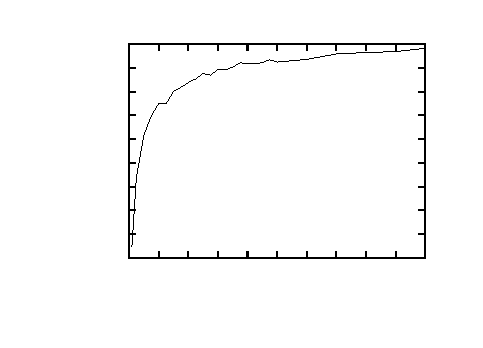
\includegraphics{info_v_trial_n}}%
    \gplfronttext
  \end{picture}%
\endgroup

\color{black} \textbf{Estimated mutual information.} Here $\sigma=1$. \color{black}
\end{center}
\end{frame}


\end{document}

